\chapter{Long Quotations}
Let's start with a long meaningless quotation so we can see how quotations are done.

\begin{quotation}
	Four score and seven years ago our fathers brought forth on this continent, a new nation, conceived in Liberty, and dedicated to the proposition that all men are created equal.
	
	Now we are engaged in a great civil war, testing whether that nation, or any nation so conceived and so dedicated, can long endure. We are met on a great battle-field of that war. We have come to dedicate a portion of that field, as a final resting place for those who here gave their lives that that nation might live. It is altogether fitting and proper that we should do this.
	
	But, in a larger sense, we can not dedicate -- we can not consecrate -- we can not hallow -- this ground. The brave men, living and dead, who struggled here, have consecrated it, far above our poor power to add or detract. The world will little note, nor long remember what we say here, but it can never forget what they did here. It is for us the living, rather, to be dedicated here to the unfinished work which they who fought here have thus far so nobly advanced. It is rather for us to be here dedicated to the great task remaining before us -- that from these honored dead we take increased devotion to that cause for which they gave the last full measure of devotion -- that we here highly resolve that these dead shall not have died in vain -- that this nation, under God, shall have a new birth of freedom -- and that government of the people, by the people, for the people, shall not perish from the earth.
\end{quotation} 
Now some text outside the quotation.
\section{Chemical Equations in \LaTeX}
If you need chemistry symbols you can use
\verb|\usepackage{mhchem}| which must be in the preamble of your main document.
They are made in the following way \verb|\ce{ H2O }| becomes \ce{ H2O }.
There is very little \ce{ O2 } in space.  
\section[Long Section Names]{Some section names are way to long to appear in the table of contents so you need to include a short title for the TOC}
This is an example of a section name that is too long.  You should shorten it if you can, but if you can't this long name will mess up the Table of Contents.  So there is an option to include a short title.  Put the short section nave version in square brackets before the actual (long) section name (in curly brackets).
Here is a random numbered list.
\begin{enumerate}
	\item one item that is long so we can see the hanging indent happen and because a hanging indent looks better, don't you think so?
	\item a second item, $2 \pi$
	
\end{enumerate}

\section{Double figures}
Sometimes it is useful to have two figures side by side. One way to do this is with a minipage environment. Here is an example of doing just that. Notice that I had to adjust the caption sizes to make the figures line up nicely. I used a \verb|\vspace| command to adjust the vertical spacing of the second figure. There are probably more elegant ways of doing this.
\begin{figure}[!htb]
	\centering
	\begin{minipage}{.5\textwidth}
		\centering
		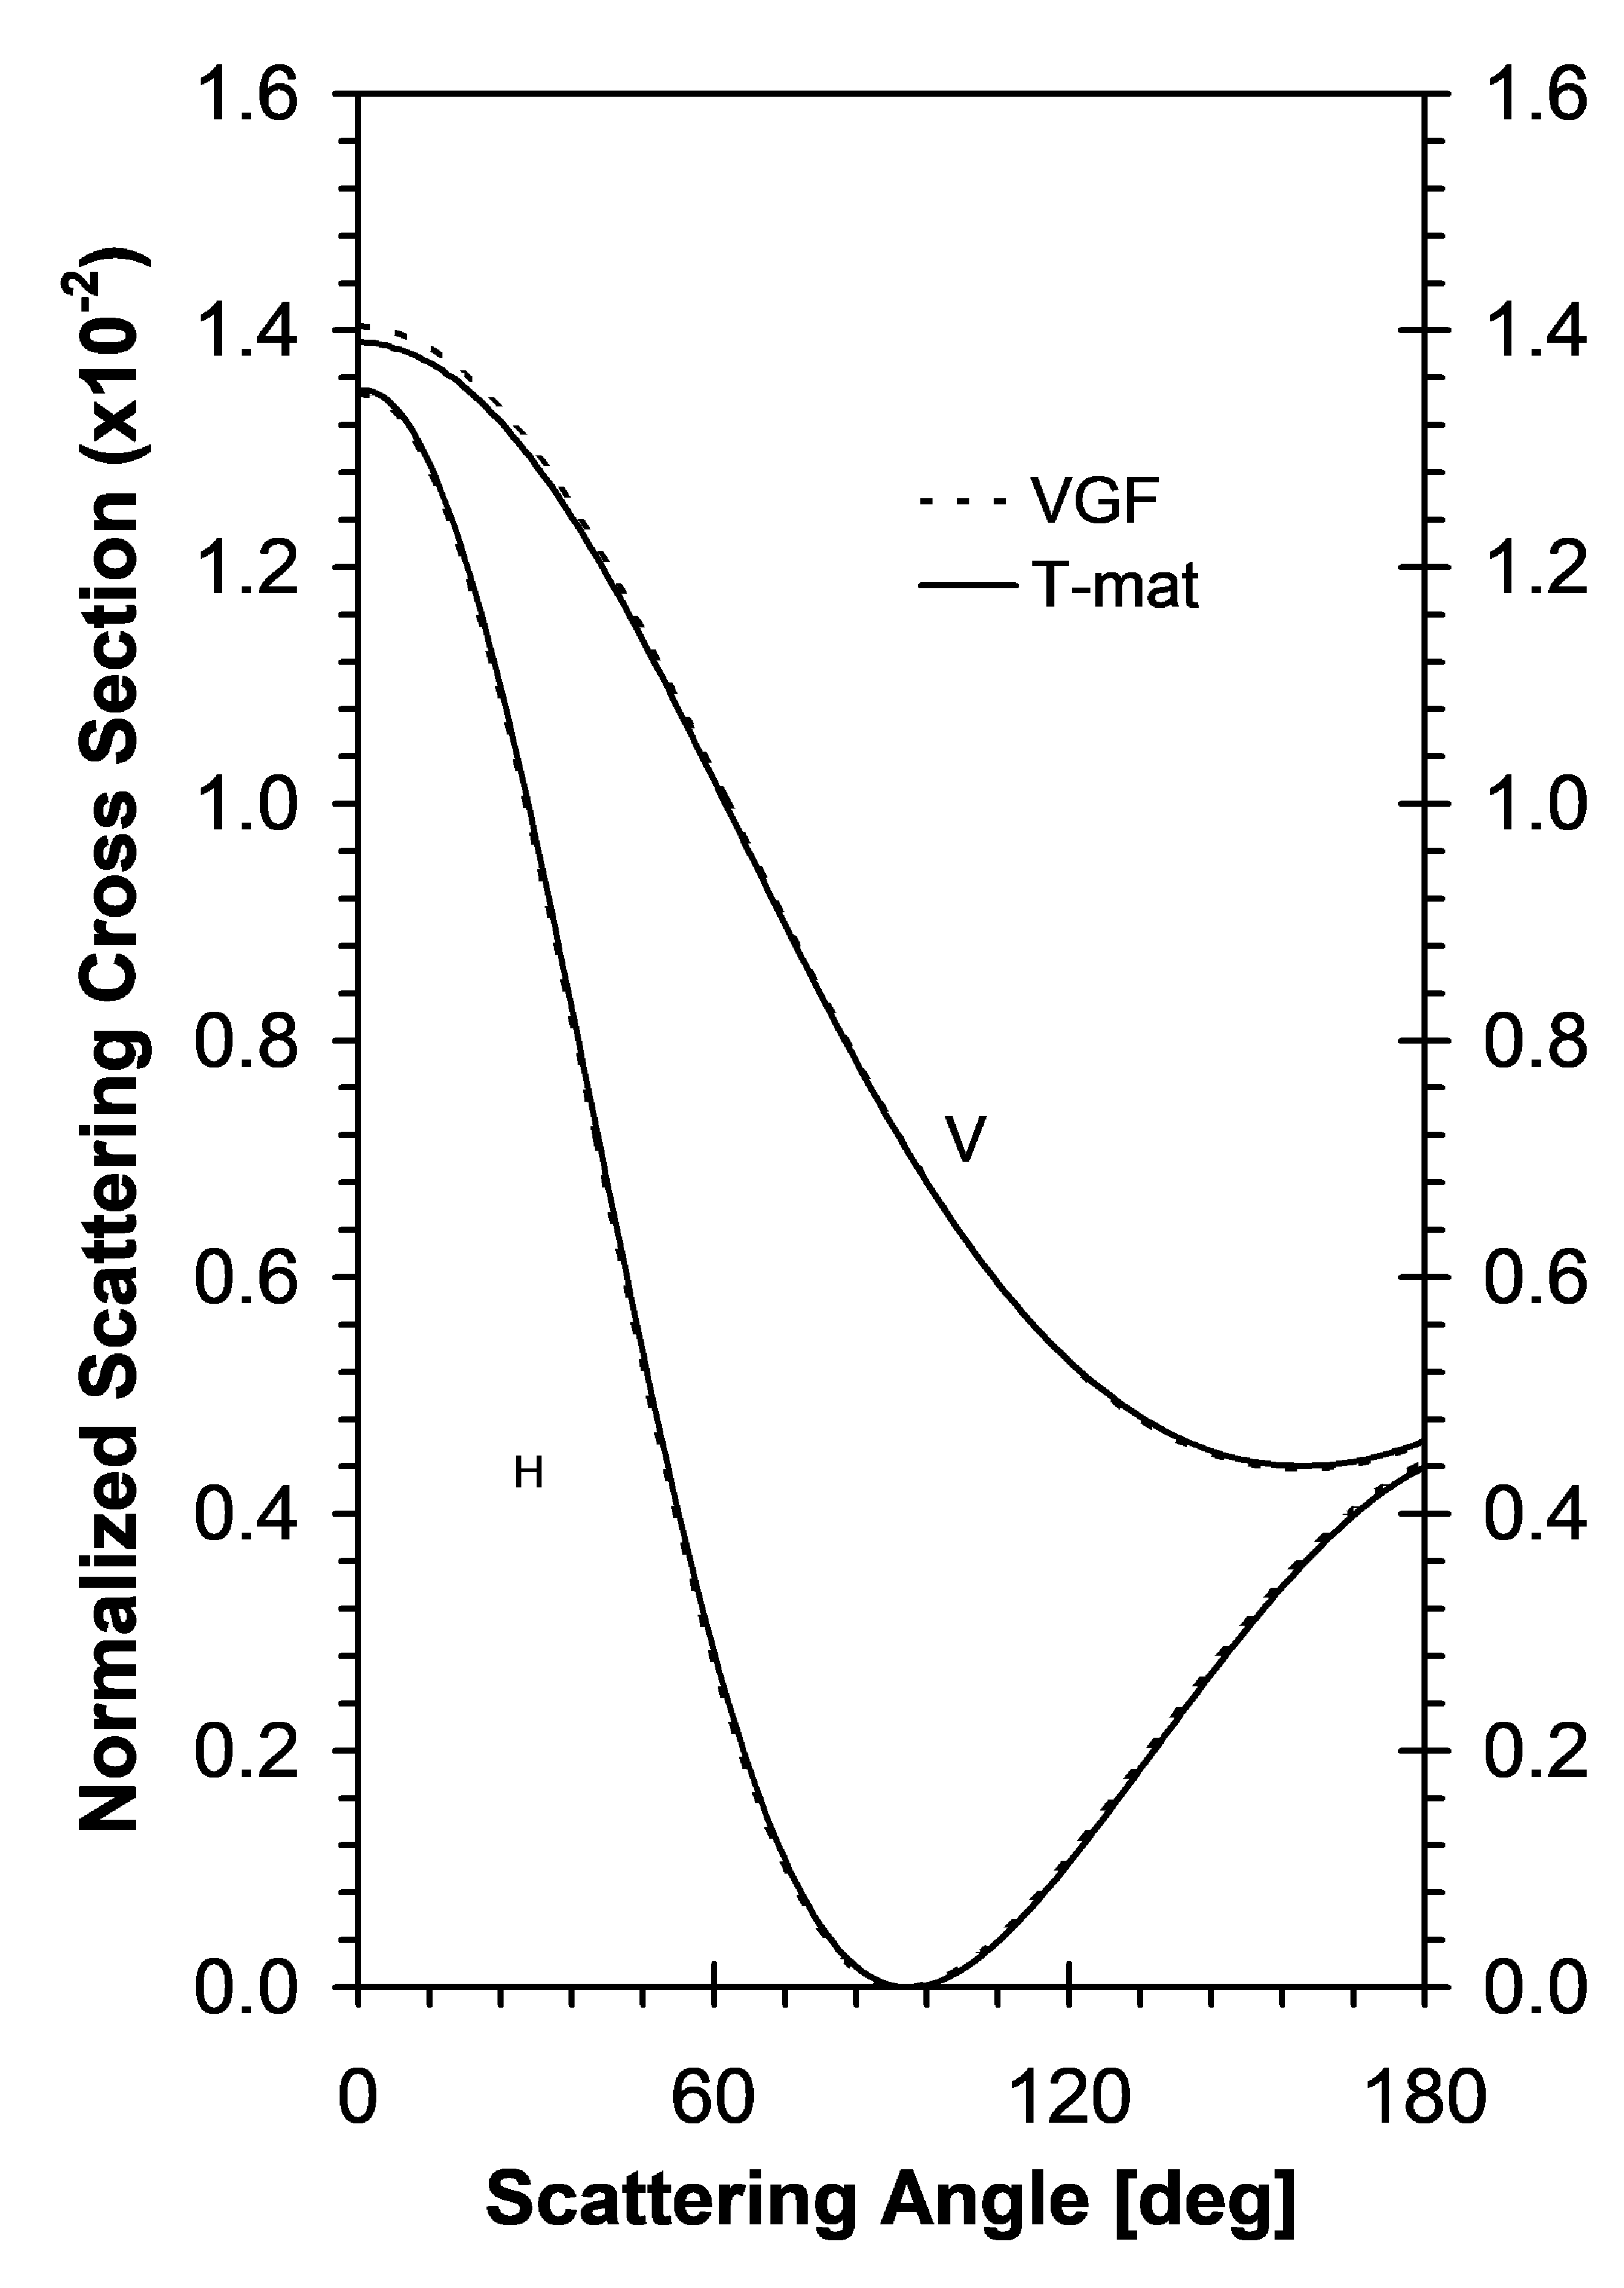
\includegraphics[width=0.8\linewidth, height=0.35\textheight]{test60b}
		\caption{Scattering From a Oblate Spheroid Rotated Once: The spheroid 
			has a semi-symmetry axis $a=1.55$ $\protect\mu m$ with $a/b=0.8,$ 
			and refractive index $m=1.2+i0.05.$ The unweighted cell length is 
			$d=0.31$ $\protect\mu m$, $N=289,$ and $\protect\lambda =10$ 
			$\protect\mu m$. Both polarizations are shown. The rotation angles 
			are $\protect\alpha =0^{\circ }$ $\protect\beta =45^{\circ },$ and 
			$\protect\gamma =180^{\circ }.$ The heavy solid curve is the VGF 
			result, the dotted curve is the T-matrix result for comparison. 
			There were 32 $k$-vectors evenly distributed in $\protect\theta$ 
			and $\protect\phi.$
		    }
	\end{minipage}%
	\begin{minipage}{0.5\textwidth}
		\centering
		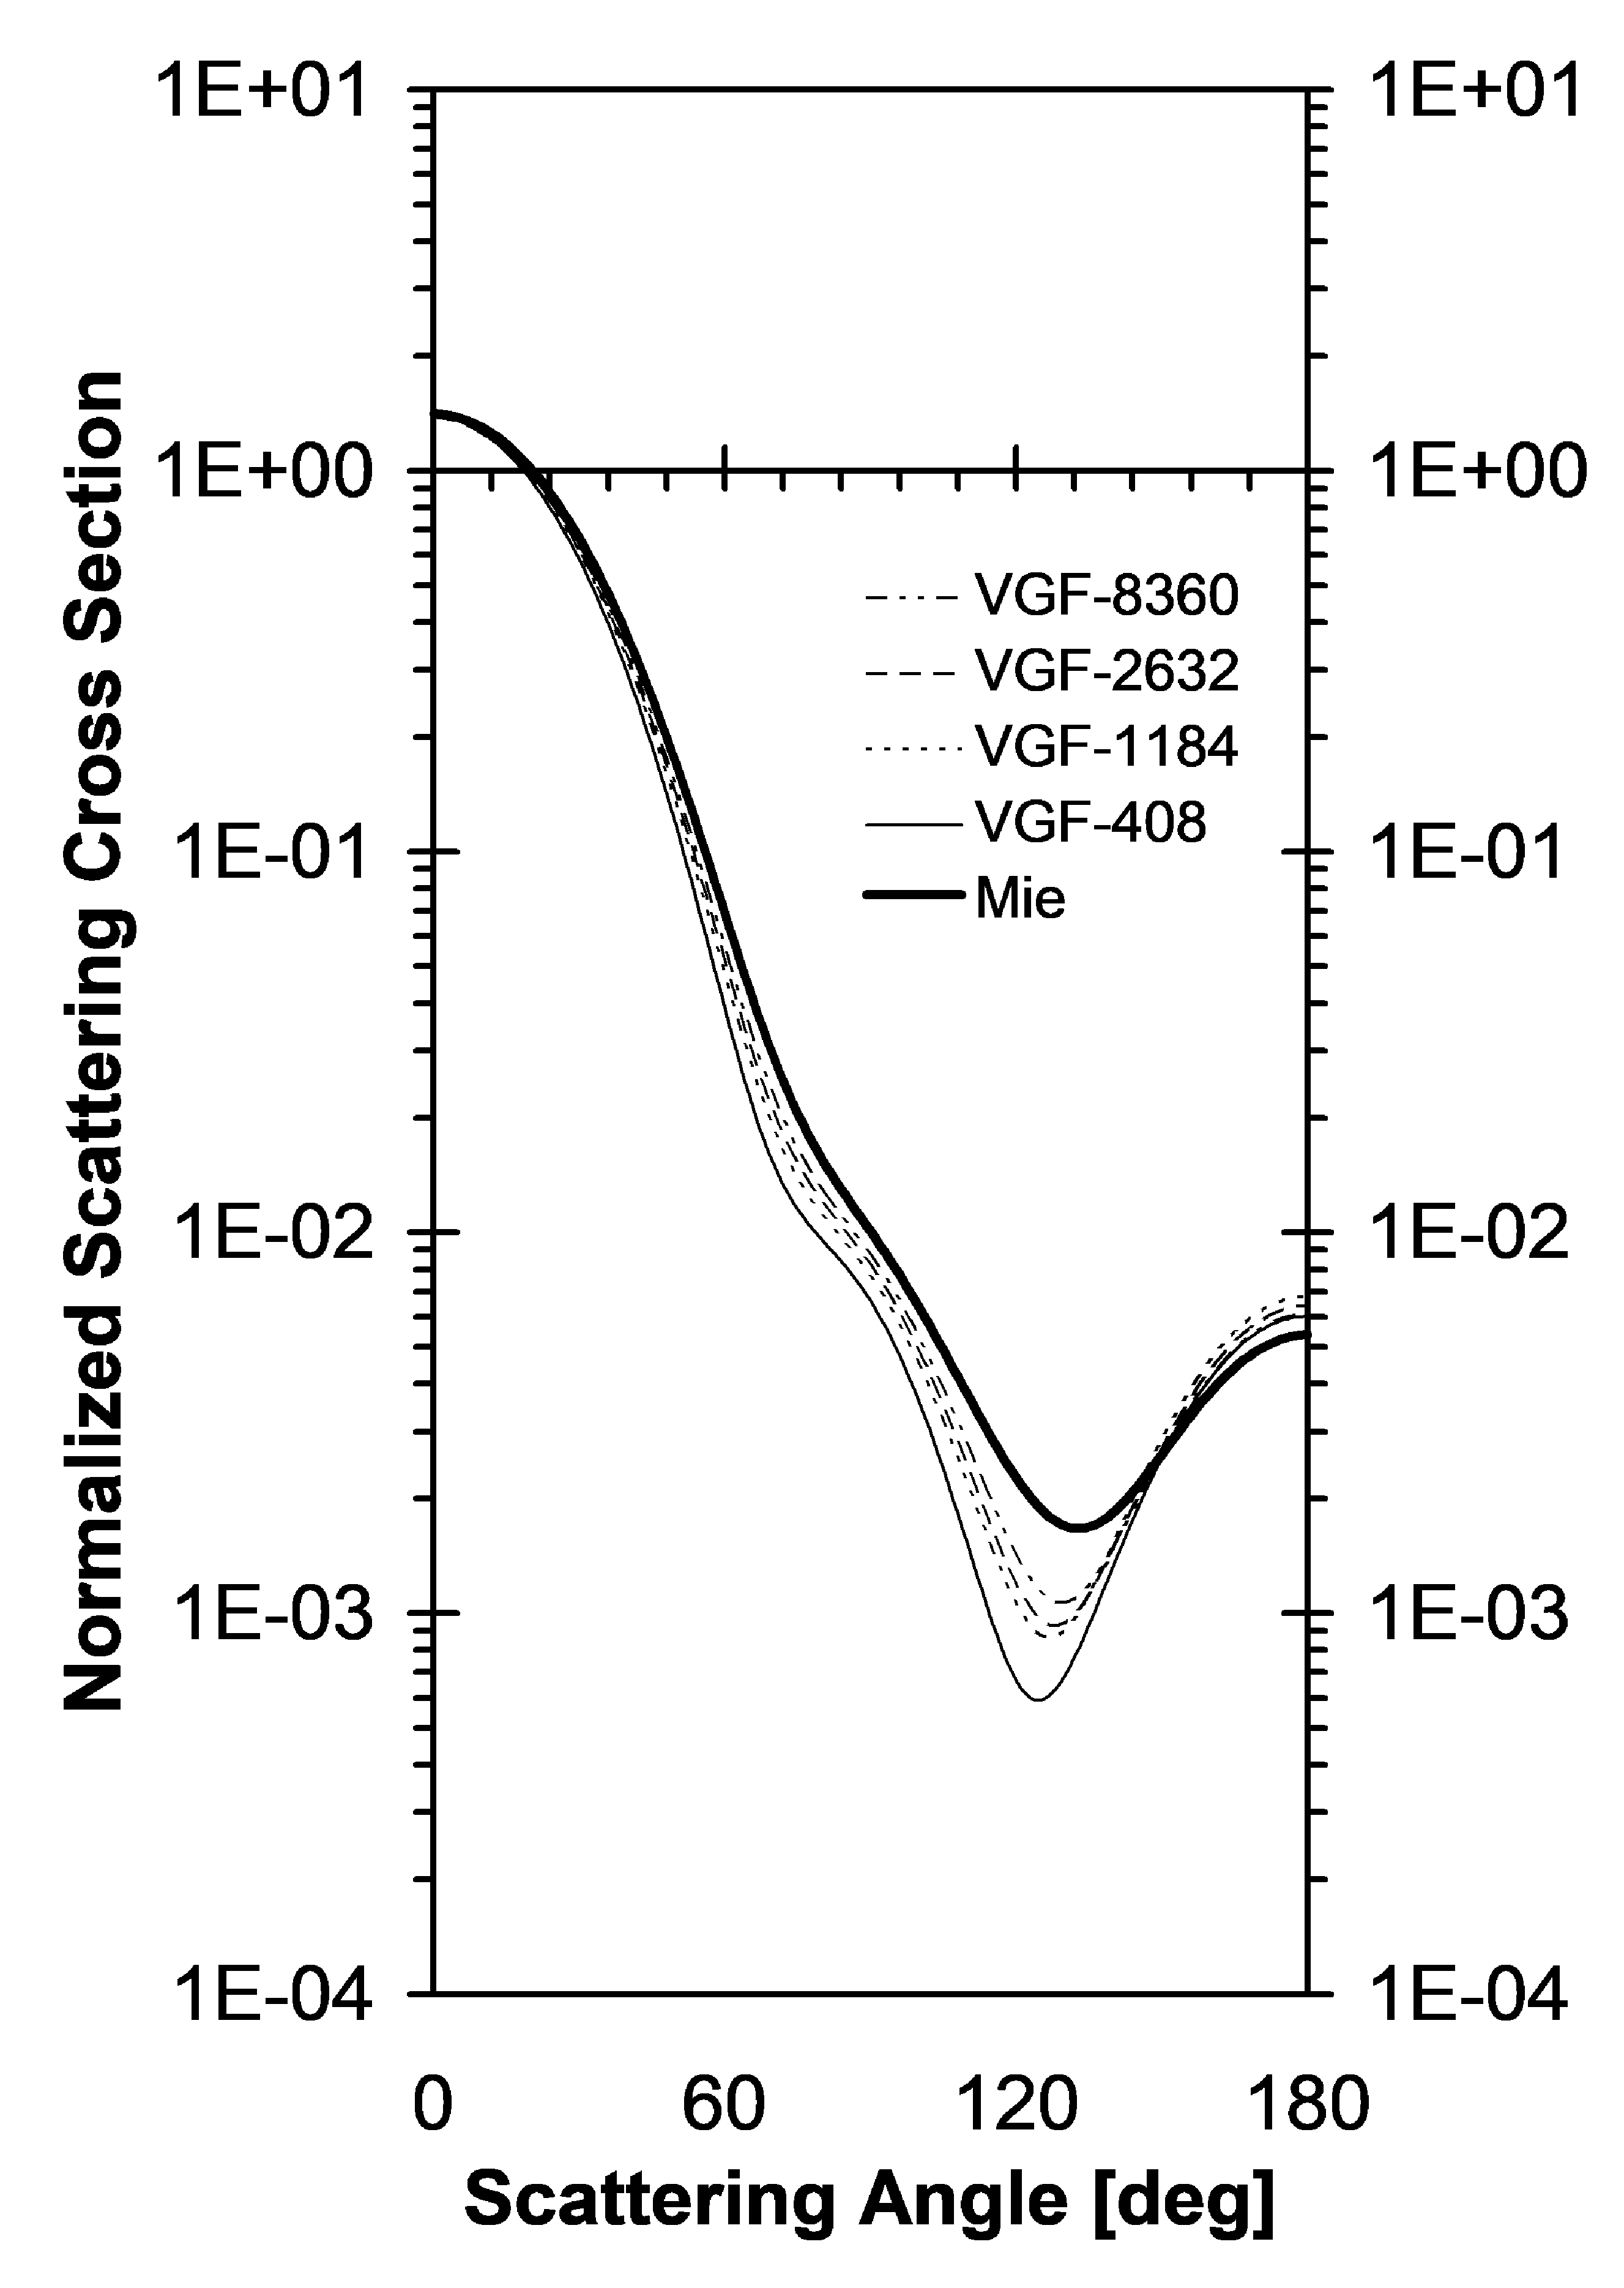
\includegraphics[width=0.9\linewidth, height=0.35\textheight]{test70}
		\caption{Scattering From a Larger Sphere: The sphere has $a=4.77$ $\protect\mu m,$ and $\protect\lambda =10$ $\protect\mu m$. Only the horizontal polarization is shown. The heavy solid curve is the Mie result. The remaining curves give VGF results for 408, 1184, 2632, and 8360 cells. \thinspace The unweighted cell size, $d$, ranges from $1.193$ $\protect\mu m$ to $0.398$ $\protect\mu m.$ There were 32 $k$-vectors evenly distributed in $\protect\theta $ and $\protect\phi.$ \vspace{0.8in}}
		\label{fig:bigsphere}
	\end{minipage}
\end{figure}
You might want to have different figures all as part of a larger figure. I recommend making the graphics as all one piece.  For example:


